\documentclass[letterpaper, 12 pt, conference]{ieeeconf}  % Comment this line out
                                                          % if you need a4paper
%\documentclass[a4paper, 10pt, conference]{ieeeconf}      % Use this line for a4
                                                          % paper
\usepackage{graphicx} 
\usepackage{caption}
\usepackage{float}
\usepackage{hyperref}
\captionsetup[figure]{font=normalsize}
\IEEEoverridecommandlockouts                              % This command is only
                                                          % needed if you want to
                                                          % use the \thanks command
\overrideIEEEmargins
% See the \addtolength command later in the file to balance the column lengths
% on the last page of the document



% The following packages can be found on http:\\www.ctan.org
%\usepackage{graphics} % for pdf, bitmapped graphics files
%\usepackage{epsfig} % for postscript graphics files
%\usepackage{mathptmx} % assumes new font selection scheme installed
%\usepackage{times} % assumes new font selection scheme installed
%\usepackage{amsmath} % assumes amsmath package installed
%\usepackage{amssymb}  % assumes amsmath package installed

\title{\LARGE \bf
Predicting Fraudulent Financial Transactions
}

\author{Aman Raj (PID:A53247556) and Anurag Paul (PID:A53271562)}


\begin{document}


\maketitle
\thispagestyle{empty}
\pagestyle{empty}


%%%%%%%%%%%%%%%%%%%%%%%%%%%%%%%%%%%%%%%%%%%%%%%%%%%%%%%%%%%%%%%%%%%%%%%%%%%%%%%%
\begin{abstract}

Applying Machine Learning for the payment industry to detect fraudulent transactions.

\end{abstract}


%%%%%%%%%%%%%%%%%%%%%%%%%%%%%%%%%%%%%%%%%%%%%%%%%%%%%%%%%%%%%%%%%%%%%%%%%%%%%%%%
\section{Introduction}

Financial fraud has become quite prevalent with the advancement of modern technology. Frauds cost customers and financial institutions millions of dollars annually which necessitate the design and development of robust fraud detection systems. However, research in this domain is quite limited due to the unavailability of open data sets due to customer privacy issues. In this project, we analyze a synthetically generated financial dataset
generated from Paysim \cite{paysim} software and develop a fraud detection system. Paysim generates synthetic datasets that resemble the normal operation of transactions and injects malicious behavior and thus provides a benchmark to evaluate the performance of fraud detection methods.

\section{Technical Approach}
In this section, we will summarize our technical approach. We give a brief overview of the dataset in Subsection \ref{subsec:dataset}. In Subsection \ref{subsec:exploration} we discuss \textbf{(a)} dataset preprocessing such as handling dataset imbalance, removing invalid entries. \textbf{(b)} analysis of fraudulent transactions to understand the relative importance of different features. \textbf{(c)} Feature engineering to generate more relevant features. We discuss different classifiers such as Naive Bayes, Logistic Regression, Linear Discriminant Analysis and Ensemble Methods to detect fraudulent transactions in Section \ref{sec:modelling}. Finally, we compare the relative performance of different models on an evaluation metric such as precision, recall, f1-score and propose the best model for fraud detection in Section \ref{sec:results}.

\subsection{Dataset} \label{subsec:dataset}
Dataset contains financial transactions generated using Paysim simulated over a span of 30 days, having following features:
\begin{itemize}
    \item \textit{step} - unit of time; 1 step is 1 hour of time
    \item \textit{type} - transaction type such as CASH\_IN, CASH\_OUT, DEBIT, PAYMENT, or TRANSFER
    \item \textit{amount} - transaction amount in local currency
    \item \textit{nameOrig} - customer starting the transaction
    \item \textit{oldbalanceOrg} - account balance before the transaction was initiated
    \item \textit{newbalanceOrig} - account balance after the transaction 
    \item \textit{nameDest} - recipient of the transaction
    \item \textit{oldbalanceDest} - balance of recipient before the transaction (not available for Merchants)
    \item \textit{newbalanceDest} - balance of recipient after the transaction (not available for Merchants)
    \item \textit{isFraud} - transactions made by the fraudulent agents inside the simulation, 0 indicates genuine and 1 indicates fraud
    \item \textit{isFlaggedFraud} - transactions which could be fraudulent wherein there is an attempt to transfer more than 200,000 in a single transaction in local currency.
\end{itemize}

\subsection{Exploratory Data Analysis}\label{subsec:exploration}
As a pre-processing step, we first fixed the naming terminology of column headers. For exploratory data analysis, we use pandas library and it's functions and try to figure out answers for the following questions.

\subsubsection{Which types of transactions are fraudulent?}
We are interested in knowing what types of transactions in the dataset are marked as fraud. In order to gain this insight, we made a bar plot of the distribution of fraudulent transactions with respect to the transaction types. As we can see from Fig. \ref{fig:transaction_type}, there are only two type of transactions namely CASH\_OUT and TRANSFER which are marked as fraudulent. Also, they are almost equal in number which can be related to the fact that possibly modus operandi of a fraudster is to first transfer the money to another account and then cashout.

\begin{figure}[ht]
    \centering
        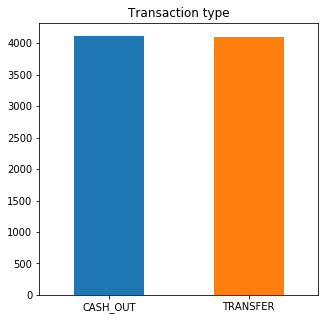
\includegraphics[width=\linewidth]{transaction_type.png}
    \caption{Transaction types where fraud is present.}
    \label{fig:transaction_type}
\end{figure}

\subsubsection{What is the correlation of different features with fraudulent transactions?}
We plot correlation among features to better understand the relationship between them, especially how do they relate to \textit{isFraud}. Also, we bin the \textit{step} feature into 24 bins from 0 to 23 referring to the hour of the day, to understand the distribution of fraudulent transactions in each hour of the day. As we can see from Fig. \ref{fig:distribution} this distribution is roughly uniform. 

After observing the correlation matrix in Fig. \ref{fig:correlation_matrix_before}, we can say that features are in general weakly correlated to \textit{isFraud}, but as we will see in later analysis together they are able to provide sufficient discriminating power.
Also, \textit{isFlaggedFraud}, \textit{step\_bin}, \textit{step} features have no correlation with \textit{isFraud} at all. So we will drop them from our further analysis.

\begin{figure}
    \centering
    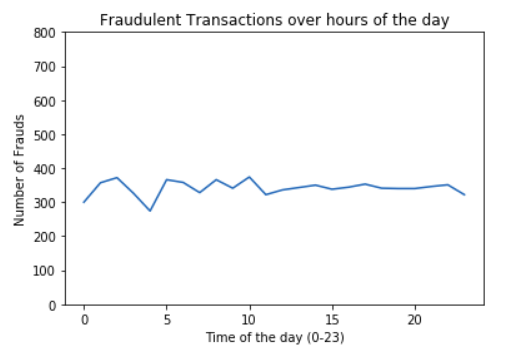
\includegraphics[width=\linewidth]{fraudvtime.png}
    \caption{Distribution of fraudulent transactions in each hour of the day.}
    \label{fig:distribution}
\end{figure}

\begin{figure*}
    \centering
    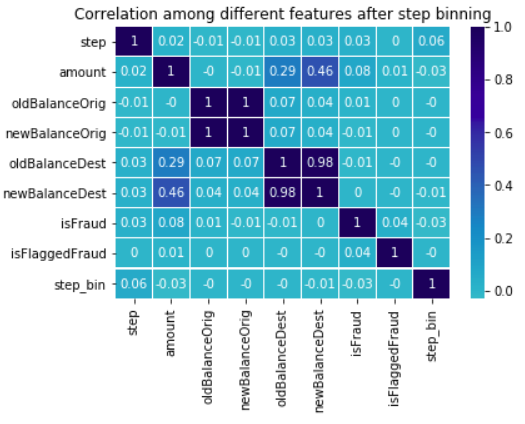
\includegraphics[width=15cm,height=15cm,keepaspectratio]{correlation_matrix.png}
    \caption{Correlation Matrix among features at the initial stage of exploration with step binning.}
    \label{fig:correlation_matrix_before}
\end{figure*}

\subsubsection{What is the significance of Merchant accounts?}
As per the dataset description, merchant accounts(whose name is prefixed by `M') should be as originators in case of CASH\_IN and as destination accounts in case of CASH\_OUT. However, in our analysis, we found this doesn't hold and merchant accounts in \textit{nameOrig} and \textit{nameDest} columns are randomly distributed.

\subsubsection{Do nameOrig and nameDest features relate to fraudulent transactions?}
From the data description and our analysis, the modus operandi for committing fraud appeared to involve first making a TRANSFER transaction to a (fraudulent) recipient who in turn cashes it out using a CASH\_OUT transaction. Thus, under this hypothesis, within this two-step process, it is expected that the fraudulent account should be present as the beneficiary account in a TRANSFER and the originator account in a CASH\_OUT. However, in our analysis, we found there are no such common accounts among fraudulent transactions. Thus, the data doesn't support the null hypothesis.

We now postulate that destination accounts for fraudulent TRANSFER`s could be originator for CASH\_OUT`s that are not detected as fraud and are labeled as genuine. If this is the case, it is possible that there may be some merit in the first hypothesis. We observed only three such transactions and from the \textit{step} information(which is information about time), for all these three transactions, genuine CASH\_OUT has occurred either way back before a fraudulent transaction took place or way after it. Therefore, we can conclude that \textit{nameOrig} and \textit{nameDest} features neither encode merchant accounts in the expected way, nor they are related to fraud modus-operandi. So, it will be safe to disregard these features from our further explorations.


\subsection{Data-Cleaning}
From the exploratory data analysis in the previous section, we know that fraud occurs only in two types of transactions - TRANSFER's and CASH\_OUT's. So we took only these types of transaction data for our next stage, for modeling classifiers to detect fraudulent transactions from given features. Also, only features that we found relevant for detecting fraud are considered in this section.

The data has several transactions with zero balances in the destination as well as originator accounts which are actually missing values for such accounts as information is not available.
So, ideally we would like to impute values for such cases. But, in our analysis we found that the percentage of fraudulent and non-fraudulent transactions where \textit{oldBalanceDest} and \textit{newBalanceDest} column set to 0 are 50\% and 0.06\% respectively. Similarly, the percentage of fraudulent and non-fraudulent transactions where \textit{oldBalanceOrig} and \textit{newBalanceOrig} column set to 0 are 0.3\% and 47\% respectively.
Hence, zero balance in destination or originator accounts is a stronger indicator for fraud, so we will not impute values for them as it will mask the fraudulent behavior in such transactions. We will replace the zero values in destination accounts with -1 which is appropriate for ML-algorithms. Also, we drop transactions having zero values in destination accounts since they don't relate to fraudulent behavior.

\subsection{Feature Engineering}
Our feature engineering is based on the fact that due to missing values there is a large proportion of transactions that are imbalanced. A balanced originator or destination account is one where the amount of transaction is equal to the difference of old and new values. Hence, we created two new features from this namely \textit{errorOrig} and \textit{errorDest} which is the difference of old and new value in account subtracted from the amount of transaction.

\begin{figure*}
    \centering
    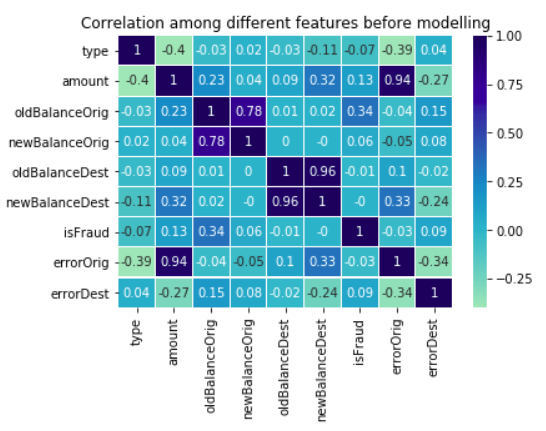
\includegraphics[width=15cm,height=15cm,keepaspectratio]{correlation_before_modelling.png}
    \caption{Correlation Matrix among features for modelling stage}
    \label{fig:correlation_matrix_after}
\end{figure*}

\section{Predictive Modelling} \label{sec:modelling}
\subsubsection{Data Splitting}
Before using machine learning algorithms, it is important to first split our dataset into train and test sub-parts so that we can train different models on the training dataset and use the test dataset to compare their generalization performance. Since we have quite a large dataset, we used 80\% of the data for training and 20\% for testing. While splitting, we ensured that the class ratio should be similar in both subparts so that test dataset can be an effective measure for testing generalization. All this is easily done in Python using \textit{train\_test\_split()} function of sklearn's \textit{model\_selection} module. 

\subsubsection{Feature Scaling}
We now perform feature scaling to ensure that our data has zero mean and close to unit standard deviation. This is required because a number of machine learning algorithms use some sort of distance metric for classification and if the values of raw data vary a lot, one feature could dominate the distance value. In addition, it has been found that gradient descent works better with normalization than without it. We use \textit{StandardScaler()} of Sklearn's preprocessing module to achieve this.

\subsubsection{Baseline Classifier}
As described above, we have a very skewed dataset, so in order to better understand the performance of the classifiers, we need to set a baseline for our evaluation metrics. We do this using \textit{DummyClassifier} from \textit{sklearn.dummy}. In case of balanced classes, we expect dummy classifier to have an accuracy of around 50\% but here we found that it achieved an accuracy of 98.86\% clearly due to the skewed nature of the data. This high value of accuracy for a dummy classifier meant that accuracy would not be a relevant metric for our project. Thus, we decided to use \textit{Average Precision Score} as the main metric to evaluate our models. As mentioned in Sklearn \cite{avgprecscore}, Average Precision Score (AP) summarizes a precision-recall curve as the weighted mean of precisions achieved at each threshold, with the increase in recall from the previous threshold used as the weight:
\begin{center}
$AP = \sum_{n} (R_{n} - R_{n-1}) P_{n}$
\end{center}
where $P_{n}$ and $R_{n}$ are the precision and recall at the nth threshold. We preferred this implementation over using the area under the precision-recall curve which is determined using the trapezoidal rule, uses linear interpolation and can be too optimistic.

% Table for rigid flow prediction
\begin{table}[htbp]
\centering
\small
\begin{tabular}{ c || c c c}
 \hline
    Classifier &  Precision & Recall & F1 \\
   \hline
  Dummy & 0.00 & 0.00 & 0.00 \\
 \hline
  Gaussian NB  & 0.16 & 0.37 & 0.22 \\
   \hline
  LDA & 0.87 & 0.38 & 0.53\\
  \hline
  Logistic Regression   & 0.88 & 0.47 & 0.61 \\
 \hline
 XGBoost & 1.00 & 1.00 & 1.00 \\
 \hline
 Random Forest & 1.00 & 1.00 & 1.00\\
 \hline
\end{tabular}
\caption{Comparison of Precision, Recall and  F1-score for class label 1 (Fraud) for various classifiers}\label{tab:comp_pr}

\end{table}

\subsubsection{Algorithms}
We used the following algorithms to identify fraudulent transactions:
\begin{enumerate}
    \item Gaussian Naive Bayes: In this method, the likelihood of the features is assumed to be Gaussian whose parameters: mean and standard deviation are estimated using Maximum Likelihood Estimation.
    \item Linear Discriminant Analysis (LDA): Instead of the features, this model fits a Gaussian likelihood to each class and classifies using Bayes Rule.
    \item Logistic Regression: In this model, the probability of each sample belonging to a class is modeled using a Logistic or Sigmoid function. Here, we use \textit{LogisticRegressionCV} which has a built-in cross-validation to determine the C parameter which is inverse of regularization strength. 
    \item Extreme Gradient Boosting (XGBoost): This algorithm learns a series of weak learners to build an ensemble that is a very powerful classifier. Here, we have used an ensemble of 100 trees with max depth 3 for each.
    \item Random Forest: In contrast to XGBoost, Random Forests learn multiple strong learners (decision trees) in parallel and average the prediction of each tree to classify. Here, we use an ensemble of 10 trees with no limit on max depth.
\end{enumerate}


\section{Result and Conclusion}\label{sec:results}
Here we present the result of our various analysis and technical approach to predictive modeling to detect fraudulent transactions.

\begin{figure}[ht]
    \centering
    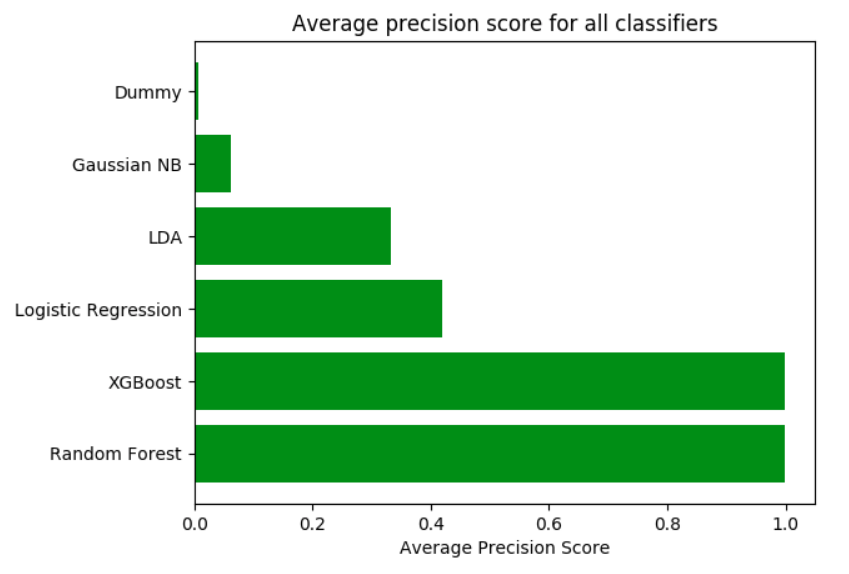
\includegraphics[width=\linewidth]{average_precision_score.png}
    \caption{Average precision score for different types of classifiers among both classes 0 and 1 averaged over different thresholds }
    \label{fig:avg_precision_score}
\end{figure}

As can be seen from the Table \ref{tab:comp_pr} and Fig. \ref{fig:avg_precision_score}, XGBoost and Random Forest are clearly outperforming simpler probabilistic models. With an almost 100\% average precision score, we feel that either of XGBoost or Random Forest can be good tools for detecting fraudulent transactions.

Through this work, we proposed a systematic approach to analyze and create statistical models to detect fraud in financial transactions which can be prevented with this knowledge.
\begin{thebibliography}{99}

\bibitem{paysim}
E. A. Lopez-Rojas, A. Elmir, and S. Axelsson. ``PaySim: A financial mobile money simulator for fraud detection". In: The 28th European Modeling and Simulation Symposium-EMSS, Larnaca, Cyprus. 2016

\bibitem{avgprecscore}https://scikit-learn.org/stable/modules/generated/sklearn.metrics
.average\_precision\_score.html

\end{thebibliography}



\end{document}
